\documentclass[12pt,a4paper]{article}
\usepackage[utf8]{inputenc}
\usepackage[german]{babel}
\usepackage[T1]{fontenc}
\usepackage{amsmath}
\usepackage{amsfonts}
\usepackage{amssymb}
\usepackage{graphicx}
\usepackage[left=2.5cm,right=2.5cm,top=2cm,bottom=2cm]{geometry}
\usepackage{float}
\usepackage{subfigure}
\author{Gruppe C14 \\ Julián Häck, Martin Koytek, Lars Wenning, Erik Zimmermann}
\begin{document}
\section{Schallgeschwindigkeit in Festkörpern, Teilversuch 2.2}
\subsection{Versuchsbeschreibung}
%Kurze Darstellung der physikalischen Grundlagen und Ziele der Versuche, die zum Verständnis des Versuches/Protokolls benötigt werden. (max. 1 Seite)
Die Ausbreitungsgeschwindigkeit v in einem Festkörper kann über den Elastizitätsmodul und die Dichte des Materials bestimmt werden:
\begin{equation}
v=\sqrt{\frac{E}{\rho}}
\end{equation}
Mit $v=f\cdot \lambda$ und $\lambda=2L$ ergibt sich für den Elastizitätsmodul:
\begin{equation}
E= \rho\cdot f^2\cdot 4L^2
\end{equation}

\subsection{Versuchsaufbau und Durchführung}
%Genaue Beschreibung der verwendeten Aufbauten unter Verwendung von Skizzen oder Photos
%Beschreibung der Messwerterfassungseinstellungen (eingestellte Messzeiten, Messbedingungen, Trigger, Anzahl der Messungen) und der Durchführung der Versuche. (max. 1 Seite)\newline
Zur Berechnung des Elastizitätsmoduls wurden 4 Stäbe mit Stativmaterial so eingespannt, dass diese nur in der Mitte einen Kontaktpunkt mit der Klemme haben (siehe Abbildung \ref{Stange}). Da wir dort einen Schwingunsknoten erwarten, können wir Verlusste durch die Aufhängung im Folgenden vernachlässigen. Nachdem wir die Massen der zylinderförmigen Stäbe bestimmt hatten und diese befestigt wurden, haben wir mehrfach die Dicken der Stangen an unterschiedlichen Stellen und die Längen gemessen. Des Weiteren konnten wir $\rho$ dann aus $\rho=\frac{M}{V}=\frac{4\cdot M}{L\cdot \pi D^2}$ bestimmen.\newline
Zur Messung der Eigenfrequenz haben wir auf das eine Stabende mit einem Gummihammer geschlagen, an dem anderen Ende wurde ein Mikrofon in ca. 5mm Entfernung angebracht, das wir mit Cassy verbunden haben. Dort konnten wir mittels Fast-Fourier-Transformation die Frequenzen bestimmen, wobei wir hier nur Grundschwingungen betrachtet haben.
\begin{figure}[H]
\centering
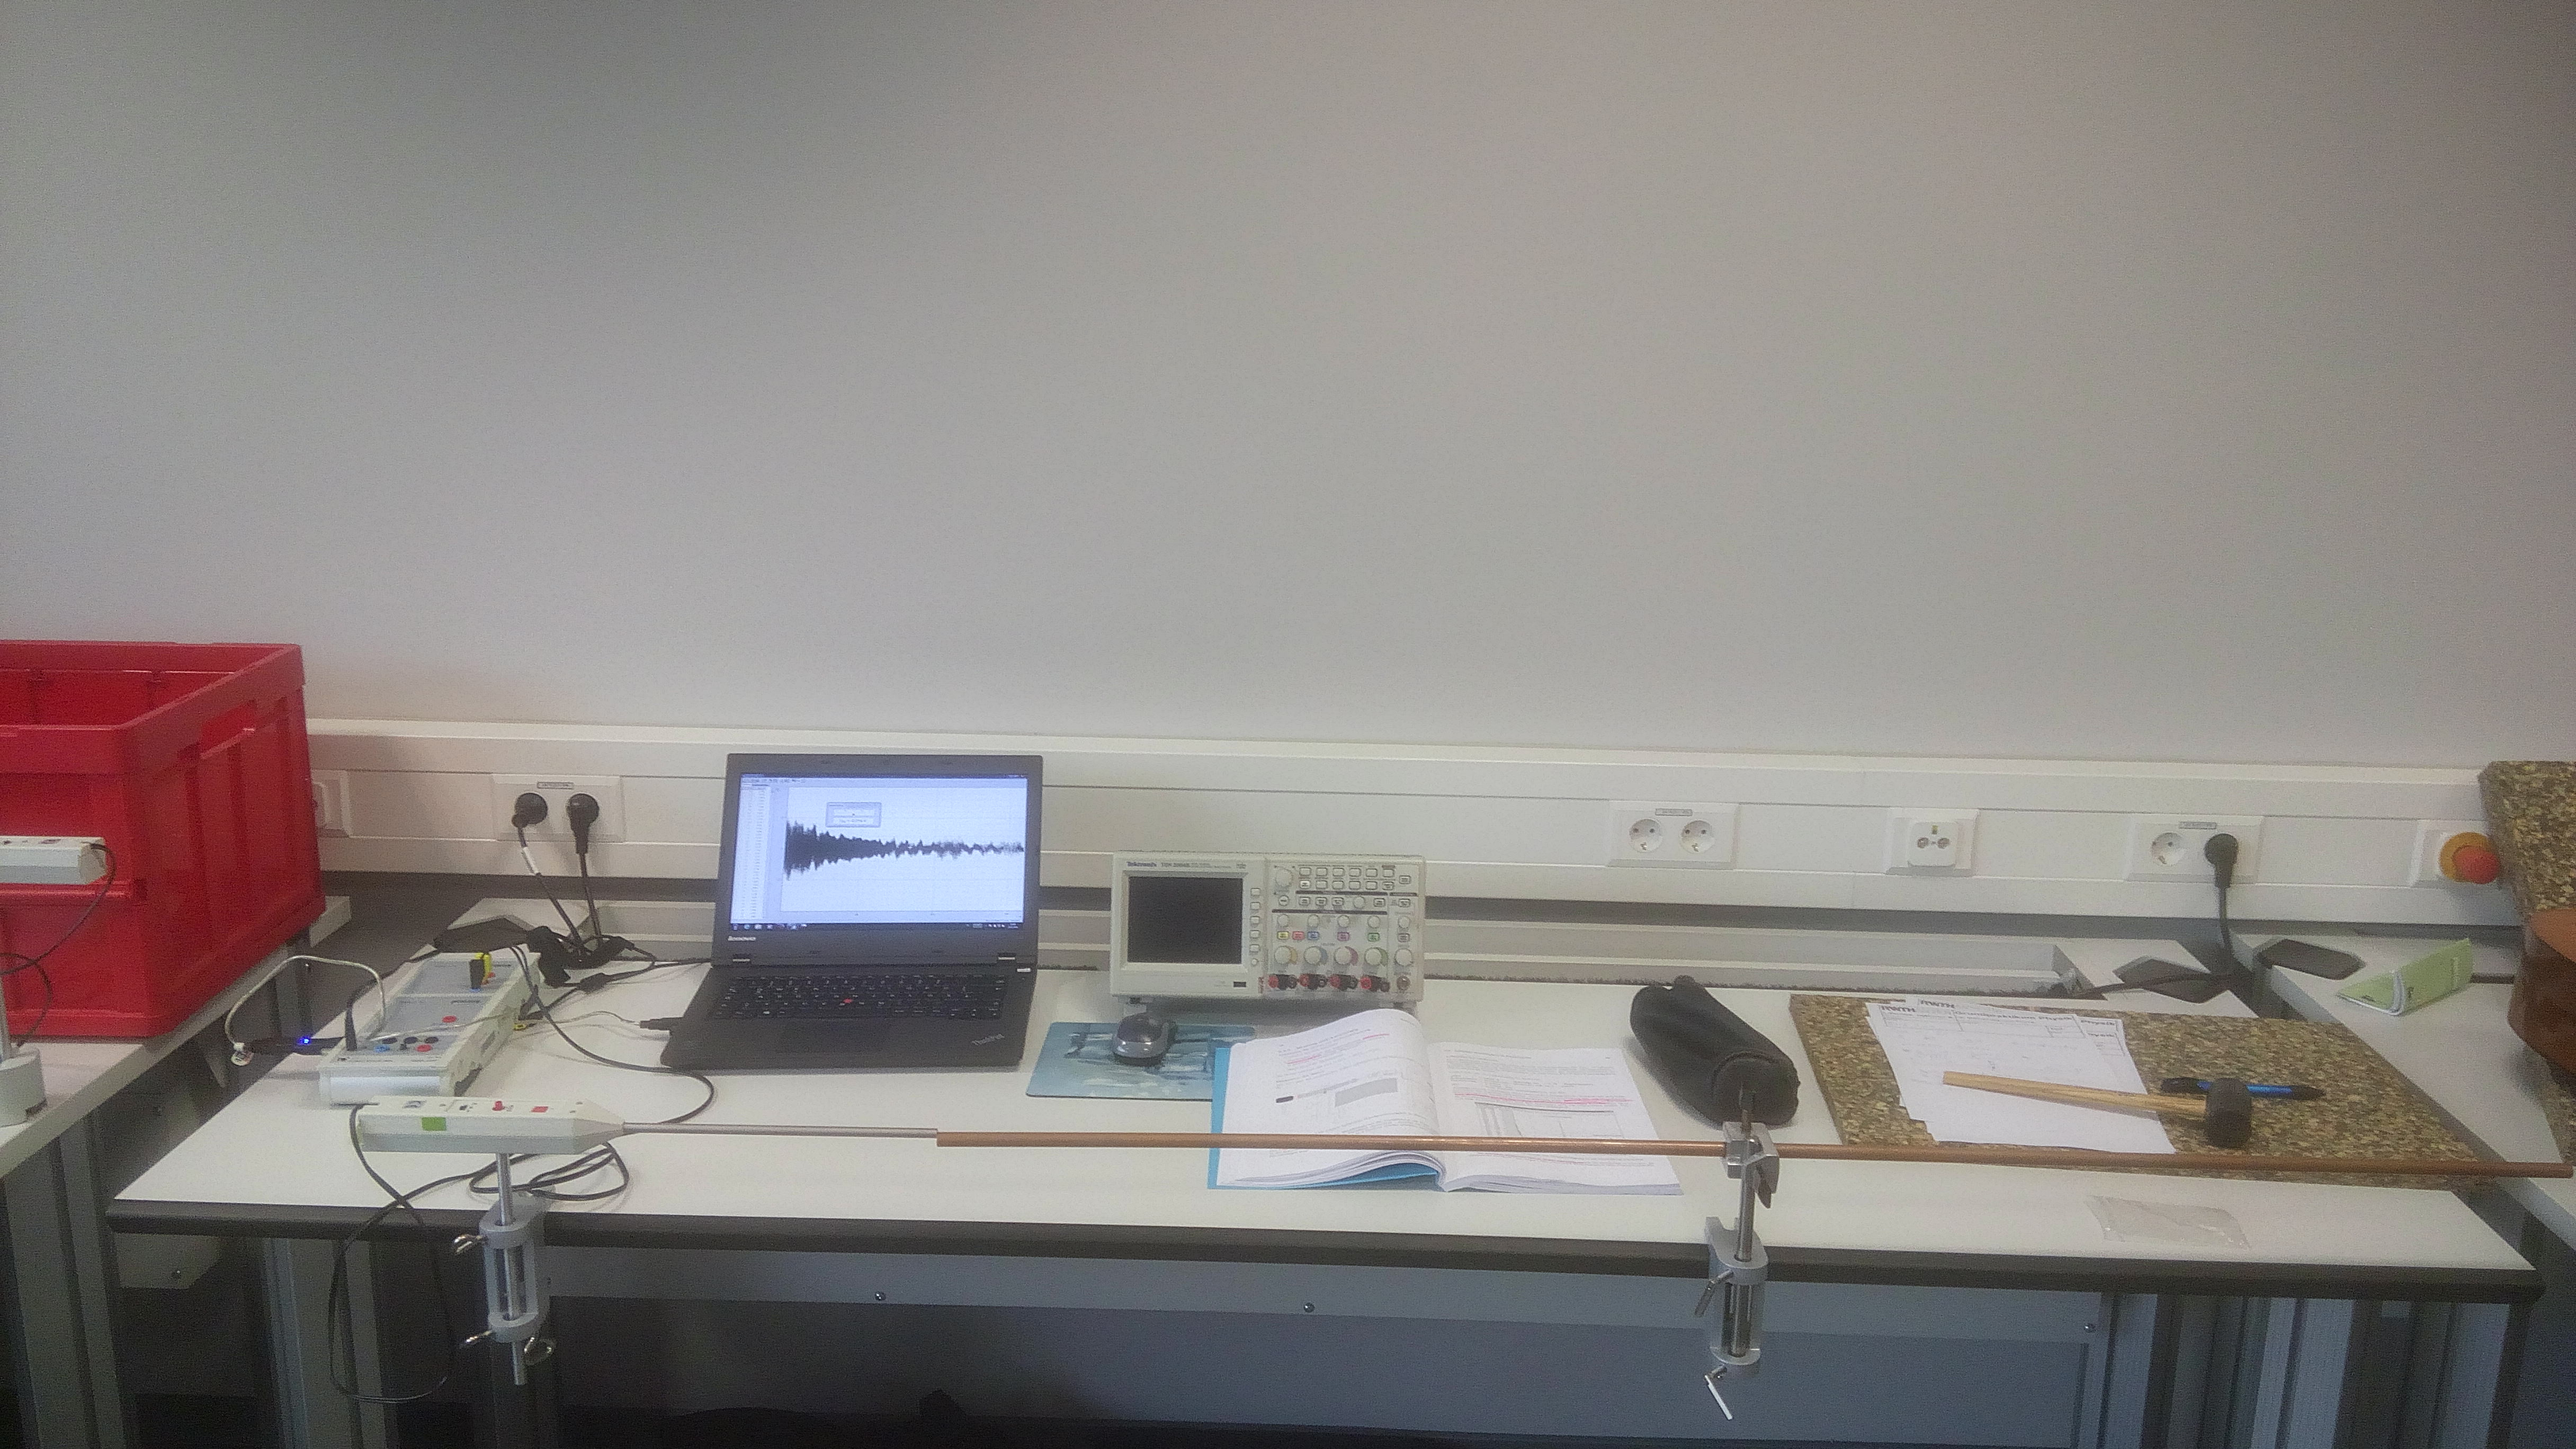
\includegraphics[scale=0.093]{Bilder/Arbeitsplatz_Stange.jpg}
\caption{Übersicht Arbeitsplatz}
\end{figure}

\begin{figure}[H]
\centering
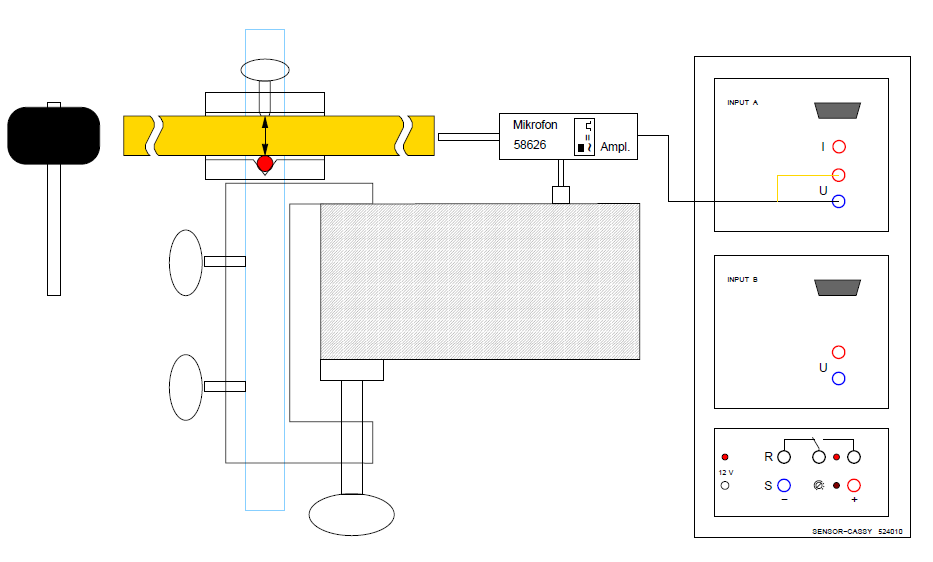
\includegraphics[scale=0.6]{Bilder/Versuchsaufbau_Skript.PNG}
\caption{Versuchsaufbau}
\label{Stange}
\end{figure}


\subsubsection{Messwerterfassungseinstellungen}
\begin{center}
\begin{tabular}{c|c}
Messbereich jeweils Messung 1-5 & -0.3..0.3V\\ 
\hline
Messbereich jeweils Messung 6-10 & -1.0..1.0V\\ 
\hline
Messintervall & 10$\mu$s \\ 
\hline
Messpunkte & 16000 \\ 
\hline
Messzeit & 1.6s \\ 
\end{tabular} 
\end{center}
Der Messbereich wurde hier immer nach der fünften Messung geändert, weil wir bei den Schlägen 6 bis 10 mit dem Stabende fester geschlagen haben und so die Amplituden in Cassy größer als der Messbereich wurden.
\subsubsection{Geräteübersicht}
\begin{itemize}
\item 4 Metallstangen
\item 1 Laptop
\item 1 Sensor-Cassy
\item 1 Universalmikrofon
\item 1 Gummi-Hammer
\item 1 Maßband
\item 1 Mikrometermaß
\item 1 Analysewaage
\item Stativzubehör
\end{itemize}
\newpage
\subsection{Versuchsauswertung}

\subsubsection{Rohdaten}

\begin{table}[H]\centering
\caption{Masse m und Länge L der Stangen}
\begin{tabular}{c|cccc}
& Stange 1 & Stange 2 & Stange 3 & Stange 4 \\ 
\hline
m in kg & 1.3019 & 1.3249 & 1.1570 & 1.2364 \\ 
L in m & 1.299  & 1.50 & 1.301 & 1.299 \\ 
\end{tabular} 
\end{table}
Der statistische Fehler auf die Einzelmessung ergibt sich zu:
\begin{align*}
\sigma_m=0.0001\,kg\\
\sigma_l=0.5\cdot10^{-2}\,m
\end{align*}
\begin{equation}
\sigma_i=\sqrt{\frac{\sum_i^n(x_i-x_{mean})^2}{n-1}}
\end{equation}
\begin{table}[H]\centering
\caption{Die Dicke d der Stangen (in mm) wurde an 5 verschiedenen Stellen gemessen.}

\begin{tabular}{c|cccc}
 & Stange 1 & Stange 2 & Stange 3 & Stange 4 \\ 
 \hline
$d_1$ & $12.47$ & $12.01$ & $11.97$ & $11.97$ \\ 
$d_2$ & $12.47$ & $12.00$ & $11.97$ & $11.97$ \\ 
$d_3$ & $12.47$ & $11.99$ & $11.95$ & $12.00$ \\ 
$d_4$ & $12.47$ & $11.99$ & $11.97$ & $11.97$ \\ 
$d_5$ & $12.47$ & $12.01$ & $11.96$ & $11.98$ \\ 
\hline
$d_{mean}$ & $12.47$ & 12.00 & 11.96 & 1198 \\ 
$\sigma_{d_{mean}}$ & $0.00$ & $4.47\cdot 10^{-3}$ & $4.00\cdot 10^{-3}$ & $5.83\cdot 10^{-3}$ \\ 
\end{tabular} 
\end{table}

Die Frequenzen f (in Hz) wurden mittels Fast-Fourier-Transformation und Peakschwerpunktbestimmung aus Cassy abgelesen.

\begin{figure}[H]
\centering
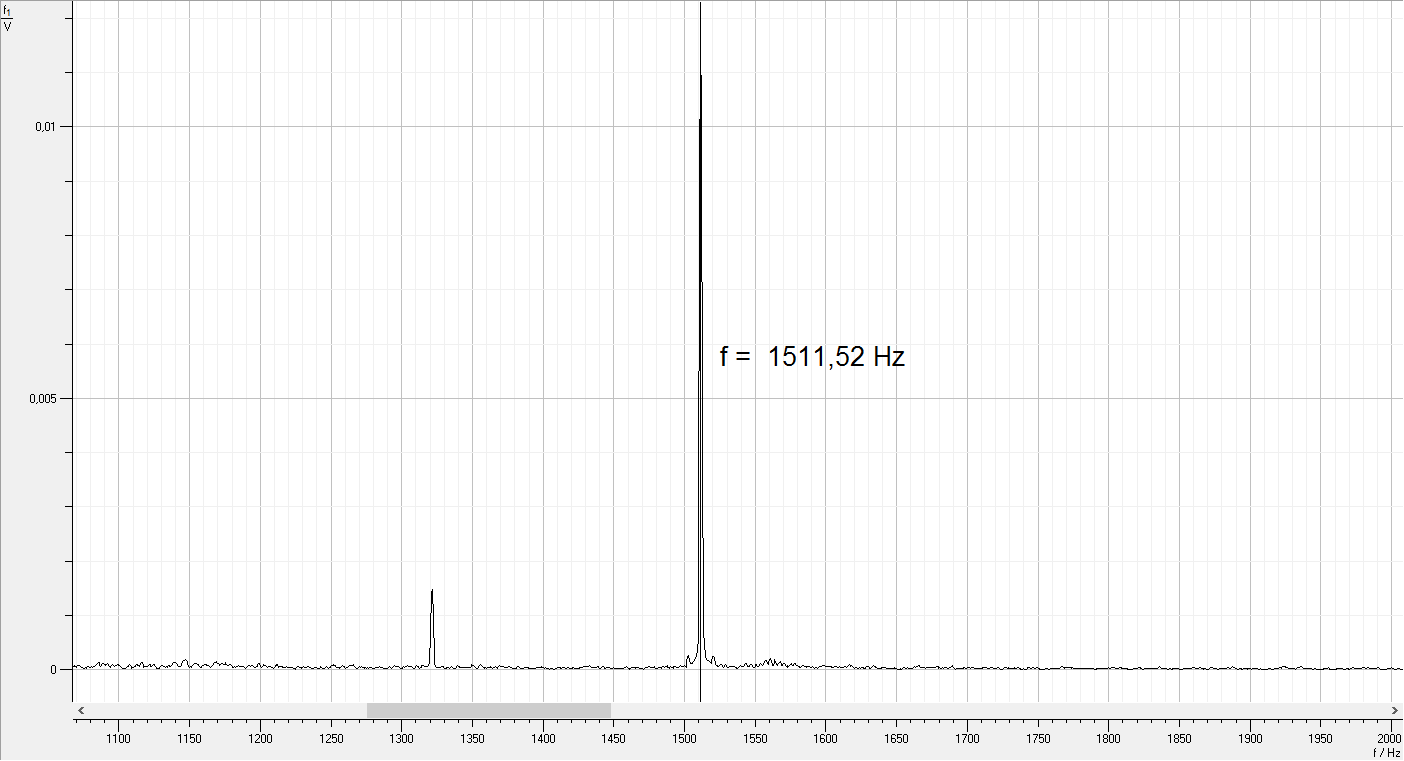
\includegraphics[scale=0.43]{Bilder/Beispiel_Cassy_Cu.png}
\caption{Beispiel zu Frequenz aus FFT ablesen (Stange 1)}
\end{figure}

\begin{table}[H]\centering
\caption{Frequenzen aus der FFT für alle 4 Stangen}
\begin{tabular}{c|cccc}
 & Stange 1 & Stange 2 & Stange 3 & Stange 4 \\ 
 \hline
$f_1$ & 1511.52 & 1728.17 & 1884.03 & 1348.48 \\ 
$f_2$ & 1511.54 & 1728.18 & 1884.04 & 1348.50 \\ 
$f_3$ & 1511.52 & 1728.18 & 1884.07 & 1348.49 \\ 
$f_4$ & 1511.53 & 1728.19 & 1884.06 & 1348.50 \\ 
$f_5$ & 1511.51 & 1728.18 & 1884.09 & 1348.50 \\ 
$f_6$ & 1511.53 & 1728.17 & 1884.11 & 1348.54 \\ 
$f_7$ & 1511.54 & 1728.18 & 1884.13 & 1348.55 \\ 
$f_8$ & 1511.51 & 1728.20 & 1884.14 & 1348.55 \\ 
$f_9$ & 1511.51 & 1728.19 & 1884.13 & 1348.52 \\ 
$f_{10}$ & 1511.48 & 1728.20 & 1884.14 & 1348.52 \\
\hline 
$f_{mean}$ & 1511.52 & 1728.18 &  1884.09 & 1348.52 \\ 
$\sigma_{f_{mean}}$ & 0.006 & 0.003 & 0.013 & 0.008 \\ 
\end{tabular} 
\end{table}

Dabei wurden die Mittelwerte mit ihren Fehlern für die Dicke der Stangen und für die Frequenzen aus
\begin{align}
x_{mean}=\frac{1}{n} \cdot \sum_i^n x_i\\
\sigma_{x_{mean}}=\frac{\sigma_i}{\sqrt{n}}
\end{align}
bestimmt.
\subsubsection{Transformation der Rohdaten und Analyse}
%Transformation der Rohdaten und Modellanpassung. (1 Seite)\\
Nachdem alle Werte in Python eingelesen wurden, haben wir die Dichten der Metallstäbe mit
\begin{equation}
\rho=\frac{M}{V}=\frac{4\cdot M}{L\cdot \pi D^2}
\end{equation}
ausgerechnet.\newline
Die Fehler auf die Dichten $\sigma_{\rho}$ ergeben sich nach Fehlerfortpflanzung zu:
\begin{equation}
\sigma_{\rho}=\sqrt{(\frac{\sigma_m}{m})^2+(\frac{\sigma_L}{L})^2+(2\cdot \frac{\sigma_d}{d})^2}\cdot \rho
\end{equation}
wobei hier nur noch mit den Mittelwerten für die Dicken gerechnet wurde, also nehmen wir einen homogenen Zylinder mit der Durchschnittsdicke $d_{mean}$ an.

\begin{table}[H]\centering
\caption{Ergebnisse der Dichten mit ihren Fehlern}
\begin{tabular}{c|cccc}
  & Stange 1 & Stange 2 & Stange 3 & Stange 4 \\ 
  \hline
$\rho$ in $\frac{kg}{m^3}$ & 8206.3 & 7809.3 & 7910.7 & 8446.8 \\ 
$\sigma_{\rho}$ in $\frac{kg}{m^3}$ & 31.6 & 26.7 & 30.9 & 33.9 \\ 
\end{tabular} 
\end{table}

Danach haben wir aus den Mittelwerten der Frequenzen, Dichten und Längen die Elastizitätsmodule der Stangen 1 bis 4 bestimmt:
\begin{equation}
E=4\rho\cdot f^2\cdot  L^2
\end{equation}
mit den Fehlern:
\begin{equation}
\sigma_{E}=\sqrt{(\frac{\sigma_{\rho}}{\rho})^2+(2\cdot \frac{\sigma_L}{L})^2+(2\cdot \frac{\sigma_f}{f})^2}\cdot E
\end{equation}

\begin{table}[H]\centering
\caption{Ergebnisse der Elastizitätsmodule mit Fehler}
\begin{tabular}{c|cccc}
 & Stange 1 & Stange 2 & Stange 3 & Stange 4 \\
\hline 
E in GPa & 126.5 & 209.9 & 190.1 & 103.7 \\ 
$\sigma_E$ in GPa & 1.1 & 1.6 & 1.6 & 0.8 \\ 
\end{tabular} 
\end{table}

Bei der Auswertung der Ergebnisse fiel uns auf, dass Stange 2 und Stange 3 sehr ähnliche Werte für die Dichten und den Elastizitätsmodul haben. Deshalb vermuten wir, dass diese aus ähnlichem oder (fast) gleichen Material bestehen. Nach weiterer Recherche ordnen wir diese beiden Stangen als Eisen ein. Bei der ersten Stange lässt sich sowohl aus E und $\rho$, als auch durch das Aussehen auf Kupfer schließen und bei der vierten Stange analog auf Messing.\newline
Abschließend haben wir aus den Werten die Schallgeschwindigkeiten in den Metallen mit
\begin{align}
v&=\sqrt{\frac{E}{\rho}}\\
\sigma_v&=\sqrt{(\frac{\sigma_f}{f})^2+(\frac{\sigma_L}{L})^2}\cdot v
\end{align}
 bestimmt und diese mit Literaturwerten\footnote{Quelle: Wikipedia} verglichen.

\begin{table}[H]\centering
\caption{Schallgeschwindigkeiten der 4 Metallstäbe mit entsprechenden Literaturwerten}
\begin{tabular}{c|cccc}
 & Stange 1 & Stange 2 & Stange 3 & Stange 4 \\ 
\hline
v in $\frac{m}{s}$ & 3926.9 & 5184.6 & 4902.4 & 3503.4 \\ 
$\sigma_{v}$ in $\frac{m}{s}$ & 15.1 & 17.3 & 18.8 & 13.5 \\ 
daraus resultierendes Material & Kupfer & Eisen & Eisen & Messing \\ 
$v_{Literatur}$ in $\frac{m}{s}$ &$\approx 4660$ & $\approx 5170$ & $\approx 5170$ & $\approx 3500$ \\ 
\end{tabular} 
\end{table}

\subsubsection{Fazit}
%Diskussion der Ergebnisse und Vergleich der erzielten Ergebnisse mit theoretischen Vorhersagen.
Insgesamt konnten wir mit unserer Messung gute Ergebnisse erziehen, die teilweise von den Literaturwerten abweichen. Diese Abweichungen erklären wir uns durch nicht ganz reines, nicht ganz homogenes Material, sowie durch die Zylindernäherung. Außerdem wurde die Temperatur(-Veränderung) außer acht gelassen. Des Weiteren schwanken die Literaturwerte auf verschiedenen Websites und wurden oft nur als Ungefährwerte angegeben, weshalb ein präziser Vergleich nicht möglich ist.

\end{document}